\begin{tikzpicture}
\clip (0,.25) rectangle (8,7.8) ;

\node[anchor=south west,inner sep=0] at (0,0) {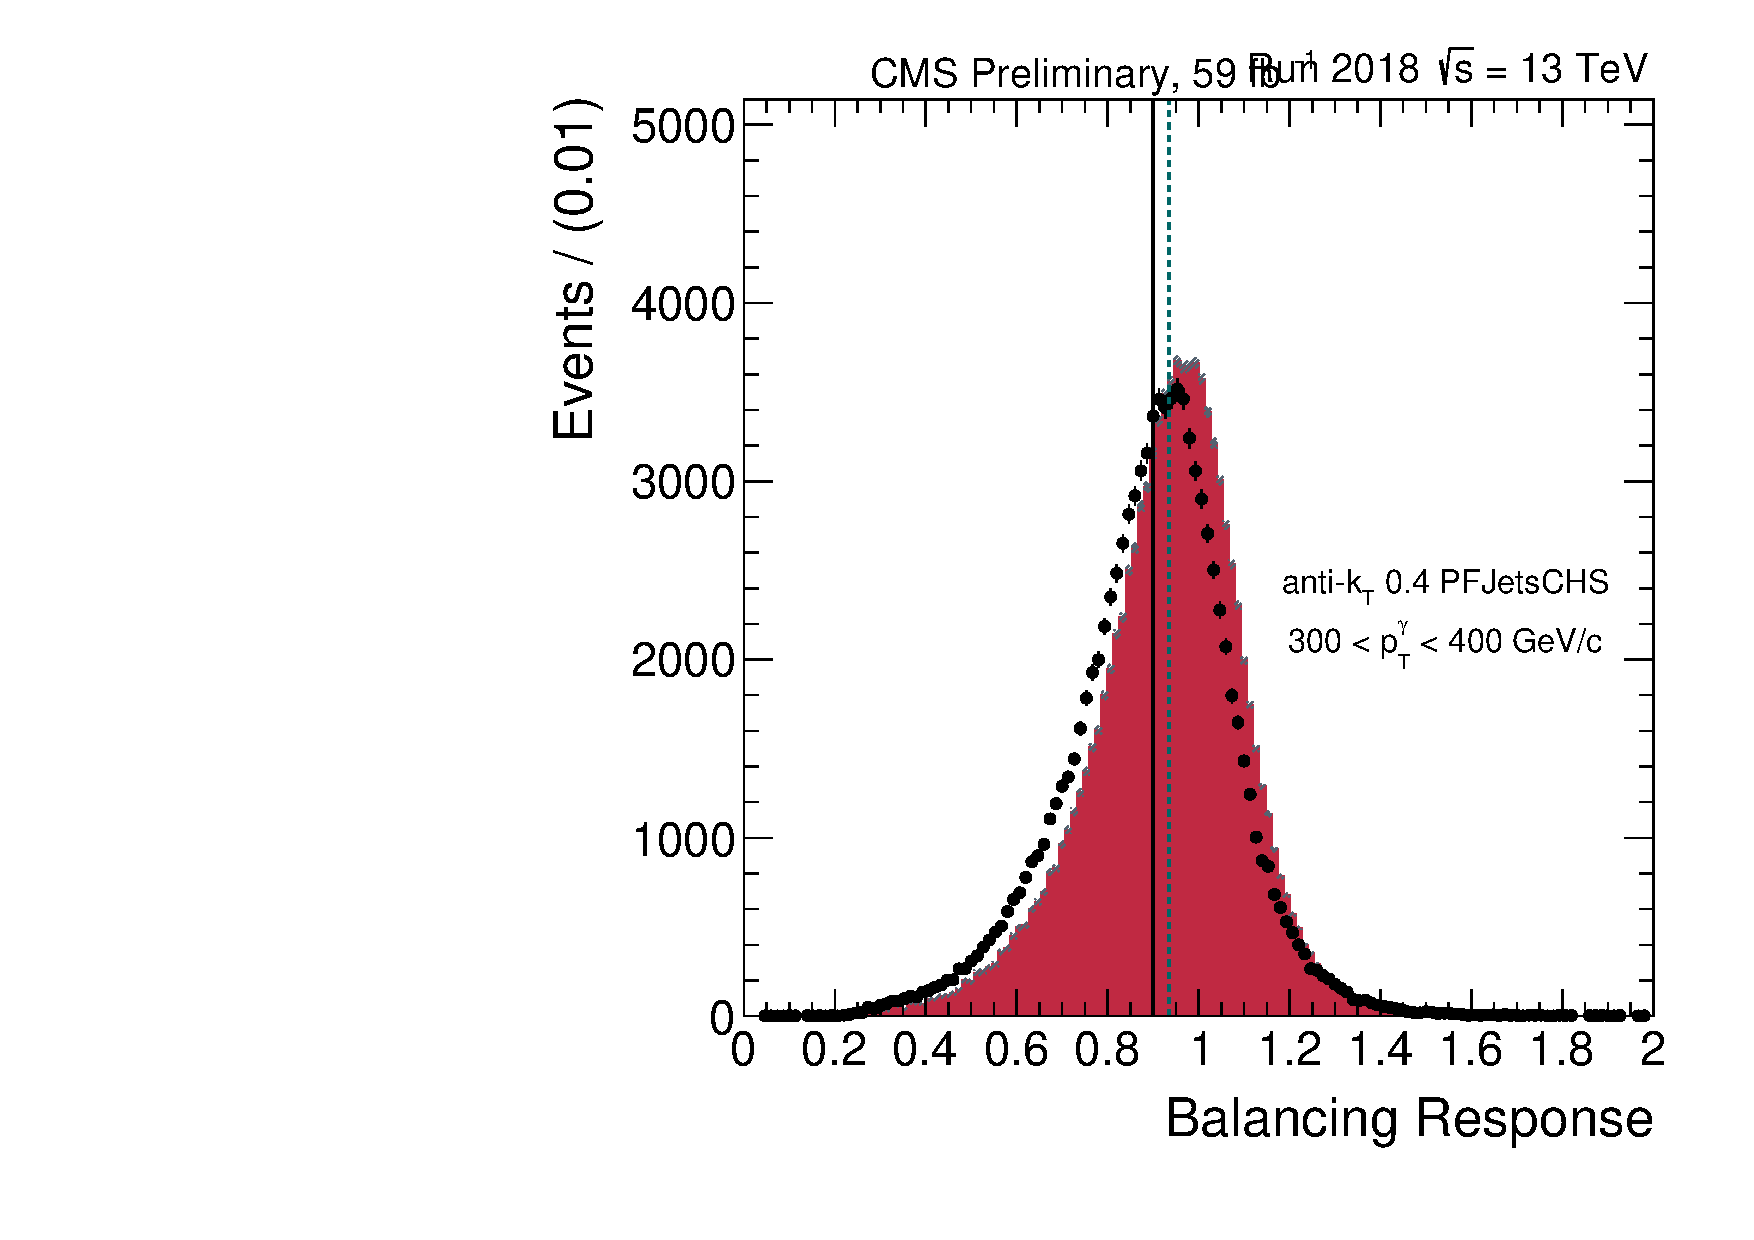
\includegraphics[width=8cm]{\PhDthesisdir/plots_and_images/my_plots/JERC/distributions/2018/source/resp_balancing_eta0013_ptPhot_300_400.pdf}};

% above txt
\fill [white] (1.2, 7.4) rectangle (7.6,7.8);
\draw (7.7, 7.6) node [left] {\footnotesize Run 2018 ABCD, \SI{59}{\femto\barn^{-1}} (\SI{13}{\TeV})};

% masks
\fill [white] (0, 0) rectangle (8,1.1);
\fill [white] (0, 0) rectangle (1.4,7.4);

% X axis
\foreach \val in {0, 0.2, 0.4, 0.6, 0.8, 1, 1.2, 1.4, 1.6, 1.8, 2}{
\draw ({1.45+(7.6-1.45)*(\val)/(2)}, .95) node {\small $\num{\val}$\vphantom{$\num{\val}\num{0.0}$}};
}
\draw (7.5, .5) node [left] {\normalsize \Rbal};

% Y axis
\foreach \val in {0, 1000, ..., 5000}{
\draw (1.5, {1.175+\val/5000*(7.2-1.175)}) node [left] {\small $\num{\val}$};
}
\draw (.25, 7.25) node [left, rotate=90] {\normalsize Nombre d'événements / \num{0.01}};

% CMS disclaimer
\draw (1.1, 7.6) node [right] {\footnotesize CMS Data};
\draw (1.7, 6.8) node [right] {\OwnWork};
\end{tikzpicture}
